\section{Einführung}

Wiederholung von letzter Woche:

\begin{definition}
    Sei $f: M \to \R$ eine glatte Abbildung, $\dim(M) = n$, $p$ ein kritischer 
    Punkt von $f$. Sei $\varphi = (x_1, ..., x_n)$ ein lokales Koordinatensystem 
    in einer Umgebung von $p$. Dann ist der \textit{Index} von $p$ die Anzahl 
    der negativen Eigenwerte von der Matrix
    \[ H_p^{\varphi}f := \left( \pdderive[f]{x_i}{x_j} \right)_{1 \leq i, j \leq n} \]
    $p$ heißt \textit{nicht degneriert}, falls  $H_p^{\varphi}f$ invertierbar ist.
\end{definition}

\begin{theorem}[Das Morse-Lemma]
    Sei $M$ eine $n$-dimensionale glatte Mannigfaltigkeit, $f: M \to \R$ glatt 
    und $p$ ein nicht degenerierter kritischer Punkt von $f$ mit Index $k$. Dann 
    existerit ein lokales Koordinatensystem $(x_1, ..., x_n)$ in einer Umgebung
    $U$ von $p$, sodass
    \[ f = f(p) - x_1^2 - ... - x_k^2 + x_{k + 1}^2 + ... + x_n^2 \]
    und 
    \[ x_1(p) = ... = x_n (p) = 0 \]
\end{theorem}
\sectiondone

Sei $M$ eine glatte Mannigfaltigkeit, $f: M \to \R$ eine glatte Abbildung, 
$a \in \R$. Dann ist $M^a = f^{-1}(- \infty, a]$ eine \textit{Subniveaumenge} 
von $f$. Eine \textit{Morse-Funktion} ist eine glatte Funktion $f: M \to \R$, 
sodass alle kritischen Punkte von $f$ nicht degeneriert sind.
Das Ziel des Vortrags ist es, die Topologie der Subnieveuamengen von 
Morse-Funktionen zu verstehen. 

Um anhand eines Beispieles die Situation zu untersuchen, benötigen wir eine 
Definition:

\begin{definition}[Eine $k$-Zelle anbringen]
    Es sei $X$ ein Topologischer Raum. Seien
    \[ e^k = D^k = \{(x_1, ..., x_k) \in \R^k: x_1^2 + ... + x_k^2 \leq 1\} \]
    \[ \varphi: \del e^k \rightarrow X \text{ stetig } \]
    \[ X \cup_{\varphi} e^k = (X \amalg e^k) / \sim, \text{ wobei } \]
    \[ \del e^k \ni x \sim y \in X \Leftrightarrow \varphi(x) = y \]
    Dann heißt $e^k$ $k$-Zelle, $\varphi$ Anheftungsabbildung 
    und $X \cup_{\varphi} e^k$ heißt $X$ mit einer $k$-Zelle 
    angebracht.
    Per Definition ist 
    \[ \varnothing \cup e^0 := e^0 = \ast \text{ und falls } X \neq \varnothing : X \cup e^0 := X \]
\end{definition}

Ein Paar Beispiele: 
\begin{itemize}
    \item Eine $1$-Zelle lässt uns Zusammenhangskomponenten mit einer "Schnur"
            verbinden, oder ist das Anheften einer "Schlaufe".
            \begin{figure}[H]
                \centering
                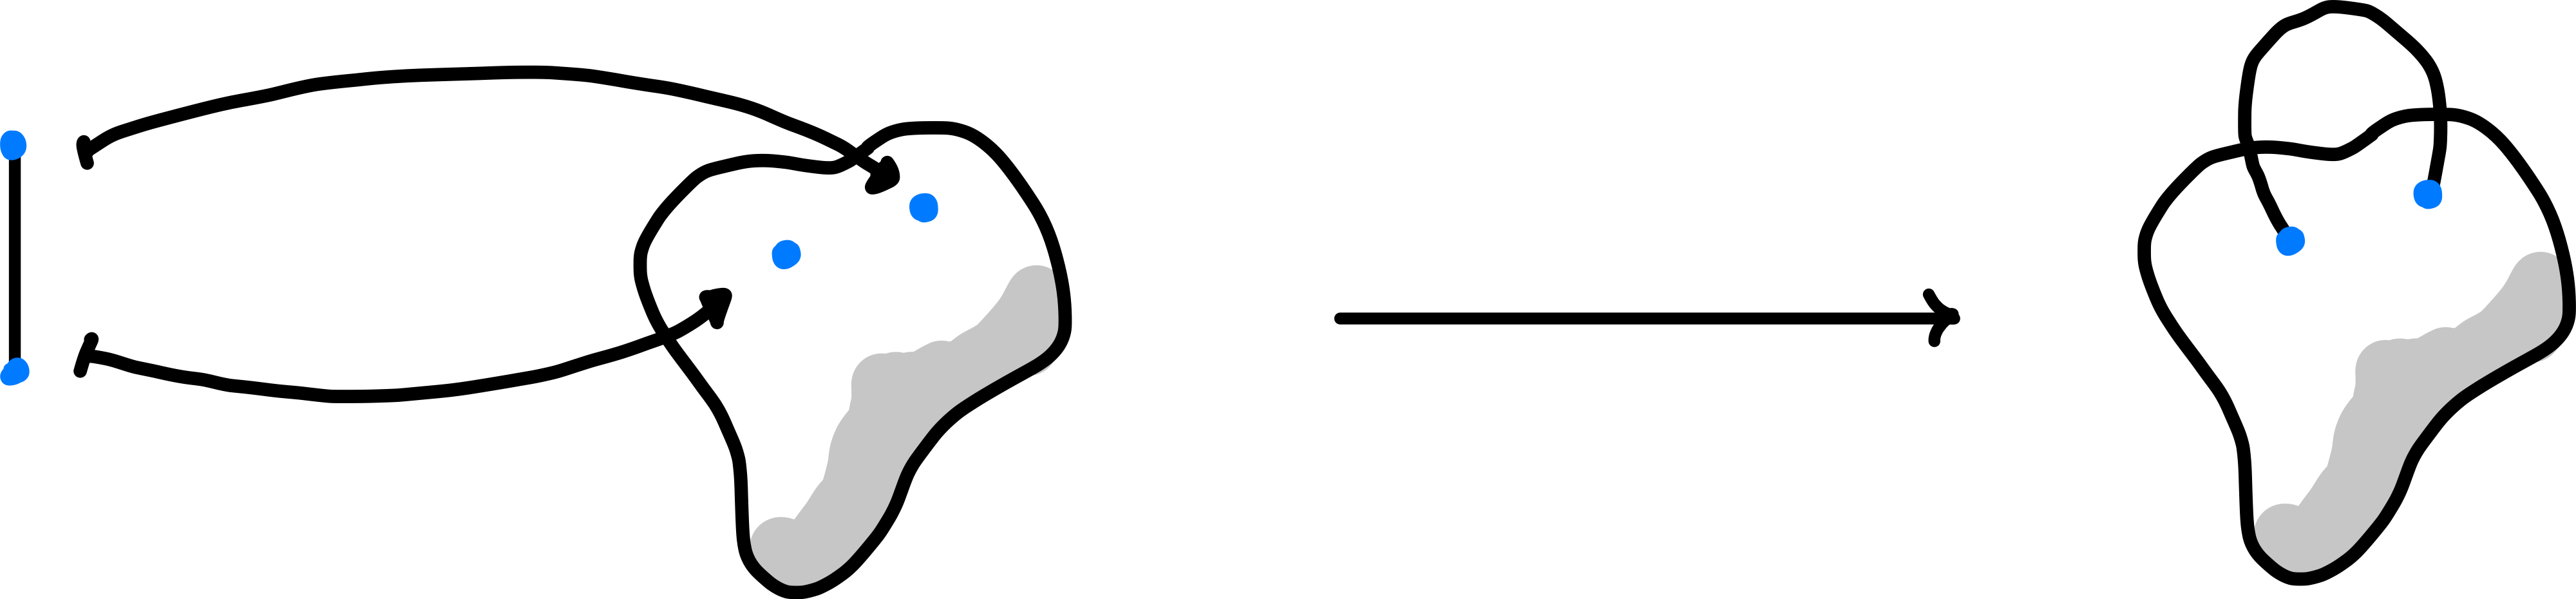
\includegraphics[width=0.45\linewidth]{resources/Me-Diagram1-attaching-a-1-cell.jpeg}
                \label{fig:me-diagram1}
            \end{figure}
    \item Eine $2$-Zelle anzubringen kann sein wie das anbringen einer Blase oder
        das stopfen eines Loches durch eine "Membran".
\end{itemize}

Wir Untersuchen die Subniveaumengen $M^a$ der Abbildung $f:M \to \R$, die den 
Punkten im Torus ihren minimalen Abstand zur eingezeichneten Ebene zuordnet:

\begin{figure}[H]
    \centering
    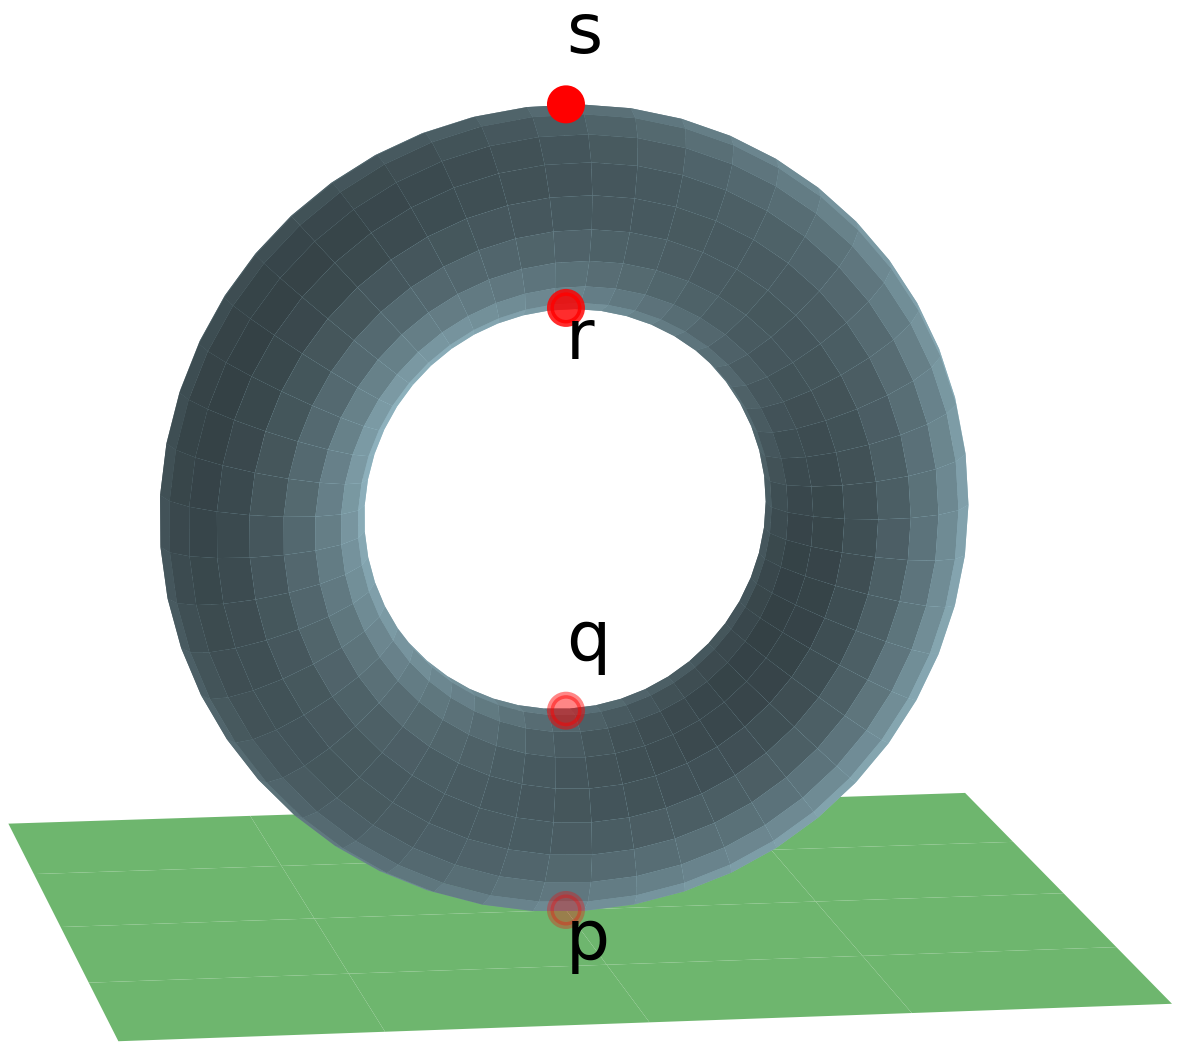
\includegraphics[width=0.6\linewidth]{resources/Me-Diagram2-torus-plane.png}
    \label{fig:me-diagram2}
    \caption{Torus auf der Ebene}
\end{figure}

Die kritischen Punkte dieser Höhenfunktion sind $p$, $q$, $r$ und $s$.

\begin{figure}[H]
    \centering
    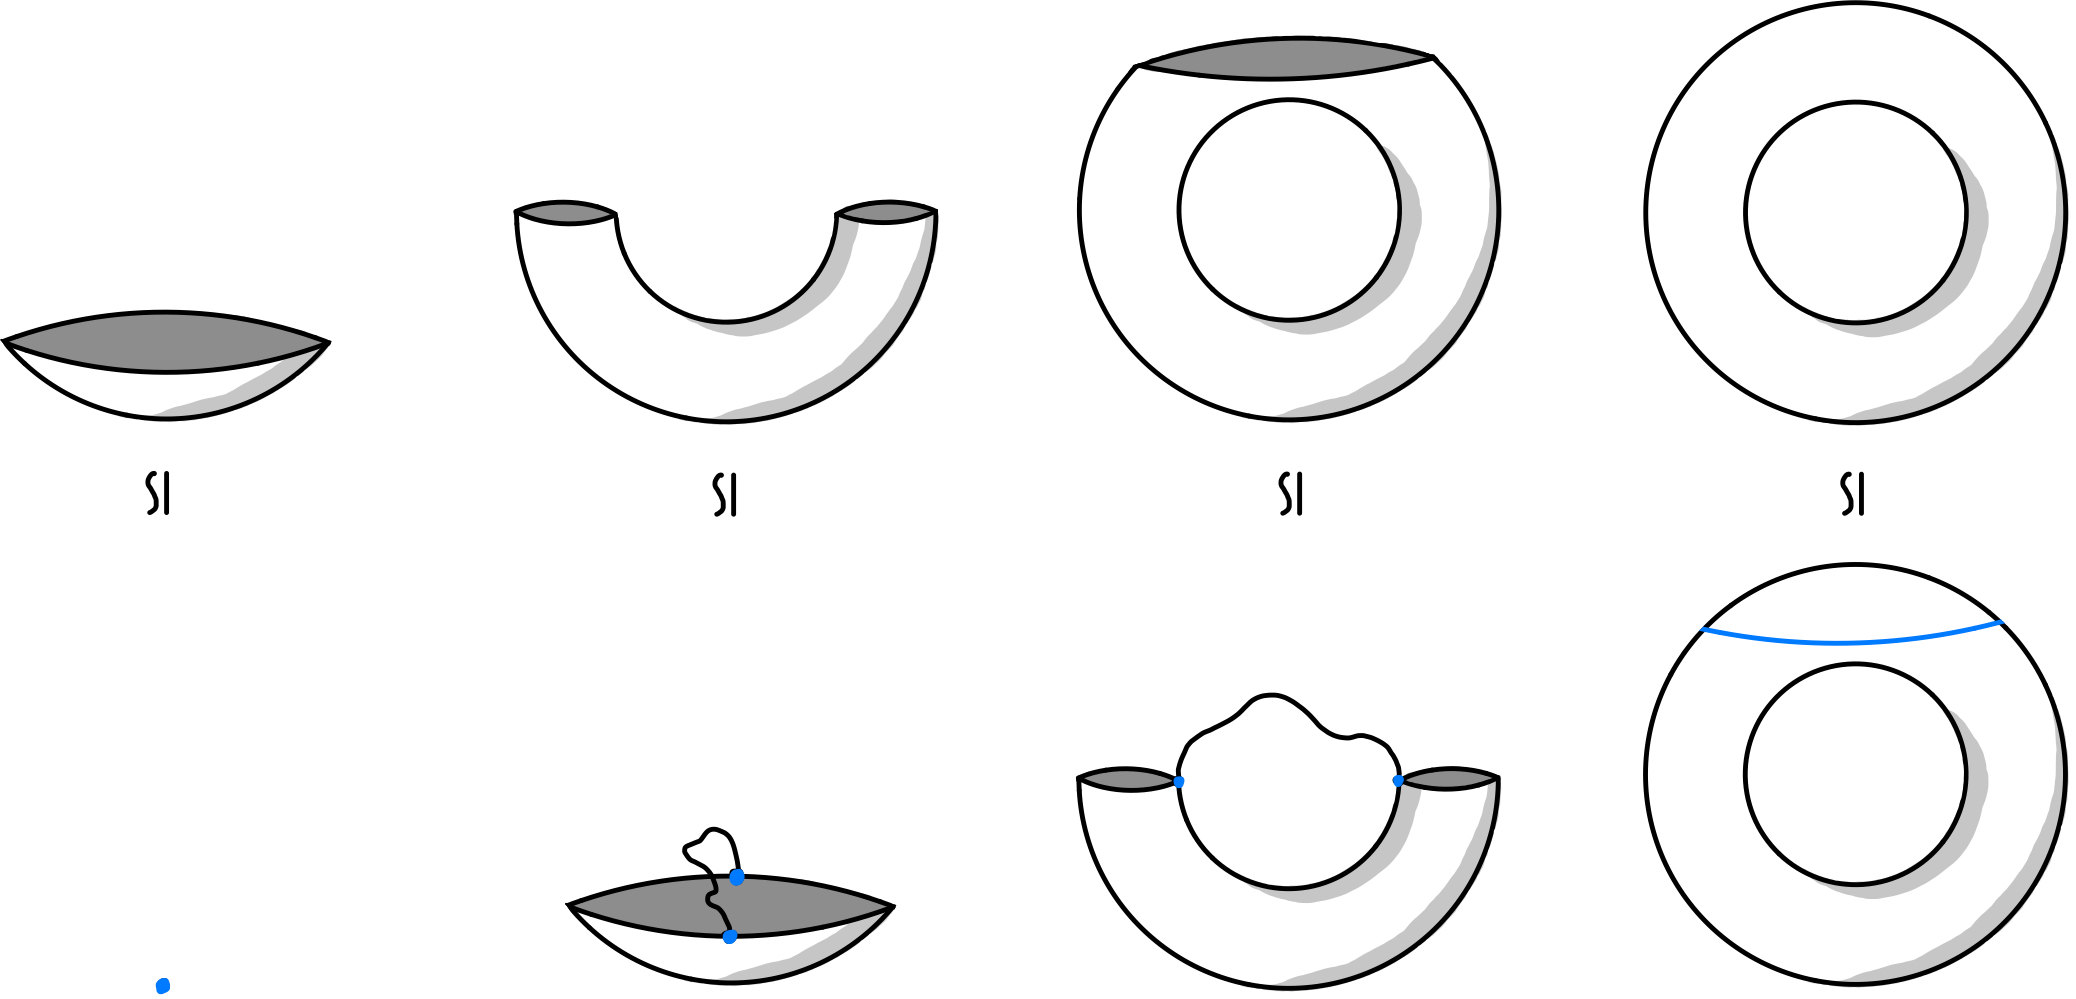
\includegraphics[width=0.8\linewidth]{resources/Me-Diagram3-torus-example.jpeg}
    \label{fig:me-diagram3}
    \caption{Niveaumengen der Höhenfunktion des Torus}
\end{figure}

\begin{itemize}
    \item Für $a < f(p)$ ist $M^a = \varnothing$.
    \item Für $f(p) \leq a < f(p)$ ist $M^a$ homotopieäquivalent zum Punkt,
        also dem leeren Raum mit einer $0$-Zelle angebracht.
    \item Für $f(p) \leq a < f(q)$ ist $M^a$ homotopieäquivalent zur vorherigen
        Subniveaumenge, an der eine $1$-Zelle angebracht wurde.
    \item Für $f(q) \leq a < f(r)$ ist $M^a$ homotopieäquivalent zur vorherigen
        Subniveaumenge, an der eine $1$-Zelle angebracht wurde.
    \item Für $f(s) \leq a$ ist $M^a$ der Torus selbst, also zur vorherigen 
        Subniveaumenge, an der eine $2$-Zelle angebracht wurde.
\end{itemize}

Wir bemerken: 
\begin{itemize}
    \item Gibt es im Intervall $[a, b]$ keine kritischen Werte, so sind $M^a$ und
        $M^b$ diffeomorph.
    \item Gibt es in $f^{-1}[a, b]$ genau einen kritischen Punkt, dann hat $M^b$ 
        den Homotopie-Typ von $M^a$ mit einer $k$-Zelle angebracht, wobei 
        $k \in \N_0$
\end{itemize}

Um diese zwei Aussagen zu präzisieren, brauchen wir einige Definitionen:

\begin{definition}[Deformationsretrakt]
    Sei $X$ ein topologischer Raum und $A \subseteq X$ ein Unterraum von $X$.
    Eine stetige Abbildung $r: X \times [0, 1] \rightarrow X$ heißt 
    \textit{Deformationsretraktion} auf $A$, falls gelten:
    \begin{align*}
        & r(\cdot, 0) = \id_X \\
        & r(X, 1) \subseteq A \\
        & r(\cdot, 1)|_A = \id_A \\
    \end{align*}
    $A$ heißt \textit{Deformationsretrakt}, falls eine Deformationsretraktion
    von $X$ auf $A$ existiert.
\end{definition}

Deformationsretrakte haben einige schöne Eigenschaften. Falls $A$ ein
Deformationsretrakt von $X$ ist, so ist die Inklusion $A \rightarrow X$ eine
Homotopieäquivalenz. Da Homotopieäquivalenz transitiv ist, hat ein weiterer
Deformationsretrakt $B$ von $X$ deshalb denselben Homotopietypen wie $A$. \\
Es ist eine Tatsache, dass zwei Unterräume $A$ und $B$ genau dan denselben 
Homotopietypen haben, wenn sie beide Deformationsretrakte eines gemeinsamen 
Oberraumes sind. Um dies einzusehen benötigt man weitere topologische 
Theorie.